\documentclass[11pt,a4j]{jsarticle}
\usepackage{float,array,booktabs,here}
\usepackage{amsmath}
\usepackage{bm}
\usepackage{listings}
\usepackage[dvipdfmx]{graphicx}
% \usepackage[whole]{bxcjkjatype}%日本語もコンパイル可にする.
%\usepackage[dvipdfmx,hiresbb]{graphicx}
\usepackage[top=25truemm,bottom=25truemm,left=15truemm,right=15truemm]{geometry}

\title{Computer Vision Final Report}
\author{81819433 開放環境科学専攻情報工学専修 修士1年 飯塚 健介}
\date{\today}
\begin{document}
    \maketitle

    \section{目的と課題設定}
    私は主にセグメンテーションについて理解を深めるために授業で習った手法を用いてセグメンテーションの処理を自分で実装して
    OpenCVに備わっているライブラリ関数での実装と比較検討、また自分の実装について考察を行った。
    今回私がセグメンテーションを選んだ理由は授業中に聞いた手法でなぜセグメンテーションができるのかが気になったからである。
    また研究として深層学習のアクセラレータの開発を行うために深層学習について調べていたときに
    セグメンテーションは自動運転や医療画像の解析などにも利用されることを知ったので応用技術としても今後ますます注目されるのだろうと考えた。



    \section{開発及び実行環境}
    開発及び実行環境は次のとおりである。OpenCVは比較と入出力を受け取るために利用した。
    \begin{itemize}
        \item OS : Ubuntu18.04 
        \item 使用言語 : Python3.6.5, C++11 
        \item 使用ライブラリ : Numpy, Matplotlib, OpenCV 
       \end{itemize}

    \section{k-means法を用いたセグメンテーション}
    まず、k-means法を用いたセグメンテーションについて検討と実装を行った。

    \subsection{k-means法について}
    アルゴリズムについて検討した。k-meansではいくつのクラスタに分類するかを人が指定しなければいけない。
    そしてランダムにクラスタリングされた3次元のベクトル(画像のRGBをベクトルの各要素とした)について各クラスタの重心を求める。
    その重心から各ベクトルのユークリッド距離を算出し最小となるクラスタに属するようにする。
    これをクラスタリング結果が前回のクラスタリング結果と一致するまで、もしくはある上限回数行い、各クラスタの重心を決定する。
    ここに新たな入力ベクトルが入ってきた場合には各クラスタの重心とのユークリッド距離を算出し最小となったクラスタに属するようにする。
    具体例として、ランダムに生成した2次元ベクトルを基にしてクラスタの重心(オレンジの四角形でプロット)を求めて、
    入力データがどのクラスタに属しているかを図\ref{fig:ex-kmeans}に示す。
    バツマークがランダムに生成したベクトル、丸マークで示しているのが入力データである。
    ユークリッド距離が一番近いクラスタに分類されているのがわかる。

    \begin{figure}[H]
        \centering
        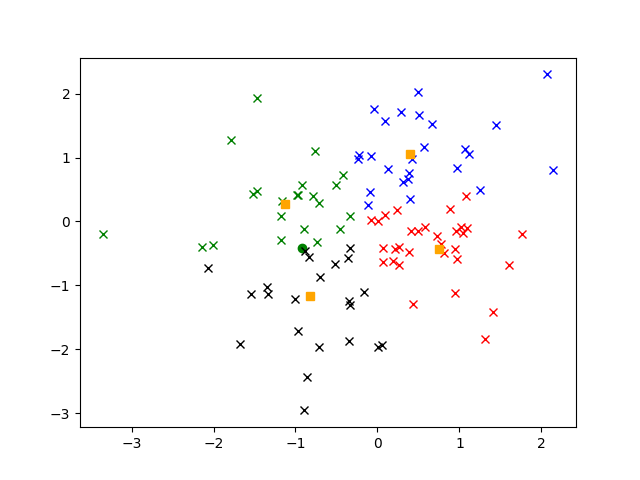
\includegraphics[clip,width=10.0cm]{img/kmeans_300.png}
        \caption{k-meansによる2次元ベクトルのクラスタリングの様子\label{fig:ex-kmeans}}
    \end{figure} 

    \subsection{実装方法}
    画像の入出力のみにOpenCVを使い、他の処理についてはnumpyの行列、ベクトル演算を自分で実装した。


    \subsection{結果と考察}
    以下に何枚かの画像について、自分で実装したk-meansでの処理結果、対象画像、OpenCVのk-meansの関数(cv2.kmeans)による処理結果を示す。
    クラスタ数はすべて8で統一した。また自分の実装、OpenCVのkmeansともに、各クラスタの色の塗り方はクラスタ重心となるRGB値を用いた。

    \begin{figure}[H]
        \centering
        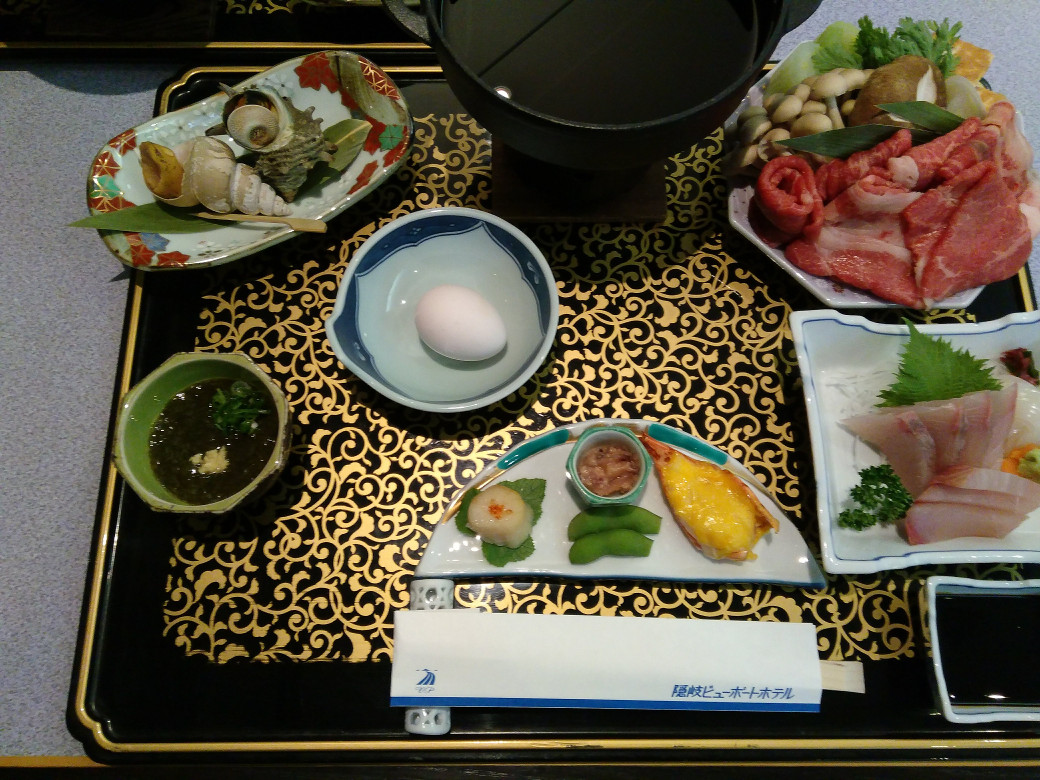
\includegraphics[clip,width=80mm]{img/good_meal.jpg}
        \caption{隠岐の島での豪華ディナーのオリジナル画像\label{fig:good_meal}}
    \end{figure} 

    \begin{figure}[htbp]
        \begin{minipage}{0.5\hsize}
         \begin{center}
          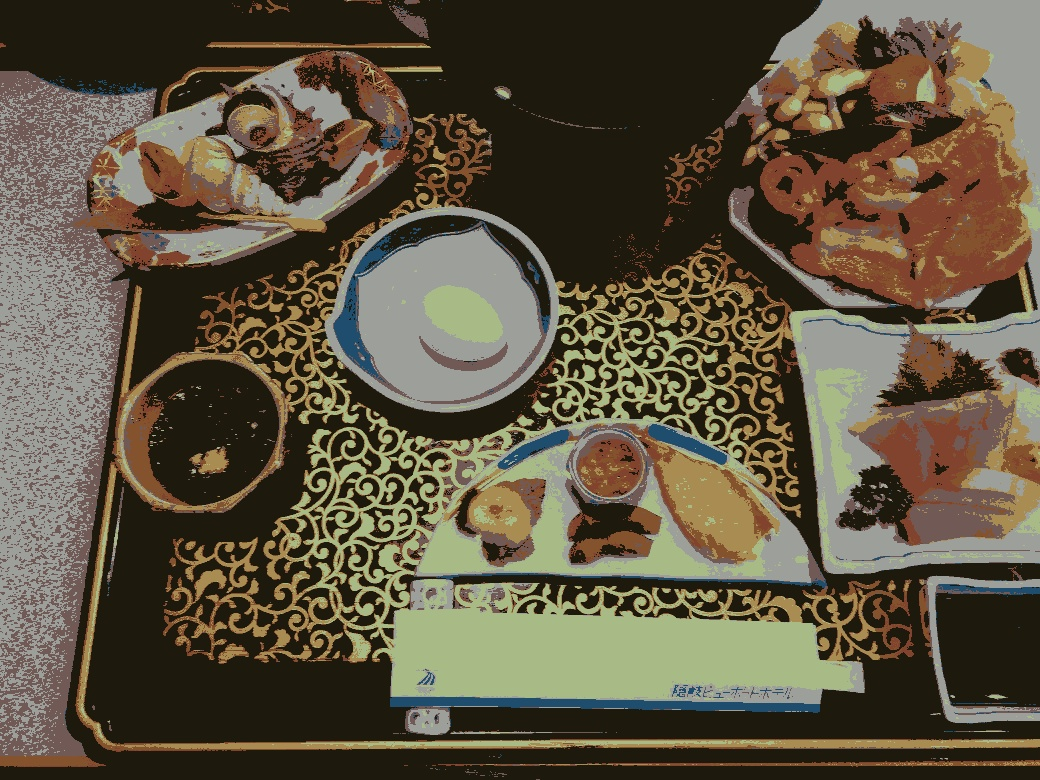
\includegraphics[width=80mm]{img/good_meal_result.jpg}
         \end{center}
         \caption{隠岐の島での豪華ディナー(自作k-means)}
        \end{minipage}
        \begin{minipage}{0.5\hsize}
         \begin{center}
          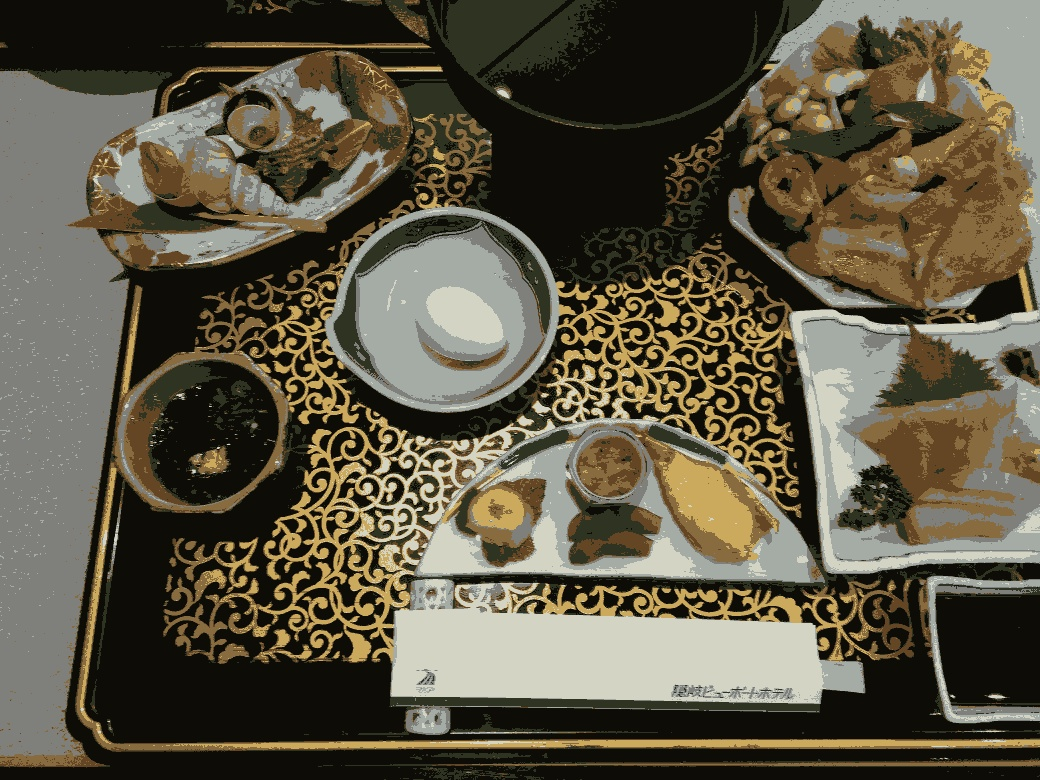
\includegraphics[width=80mm]{img/good_meal_opencv.jpg}
         \end{center}
         \caption{隠岐の島での豪華ディナー(cv2.kmeans)}
        \end{minipage}
    \end{figure} 
    自作したk-meansとライブラリのもので違いがあるが、この画像の場合には自作のもののほうがより色味を再現できている。
    お肉の赤みやお皿の青い模様などをそのまま残している。しかし野菜などの緑色はライブラリのもののほうが色味を残している。

    \begin{figure}[H]
        \centering
        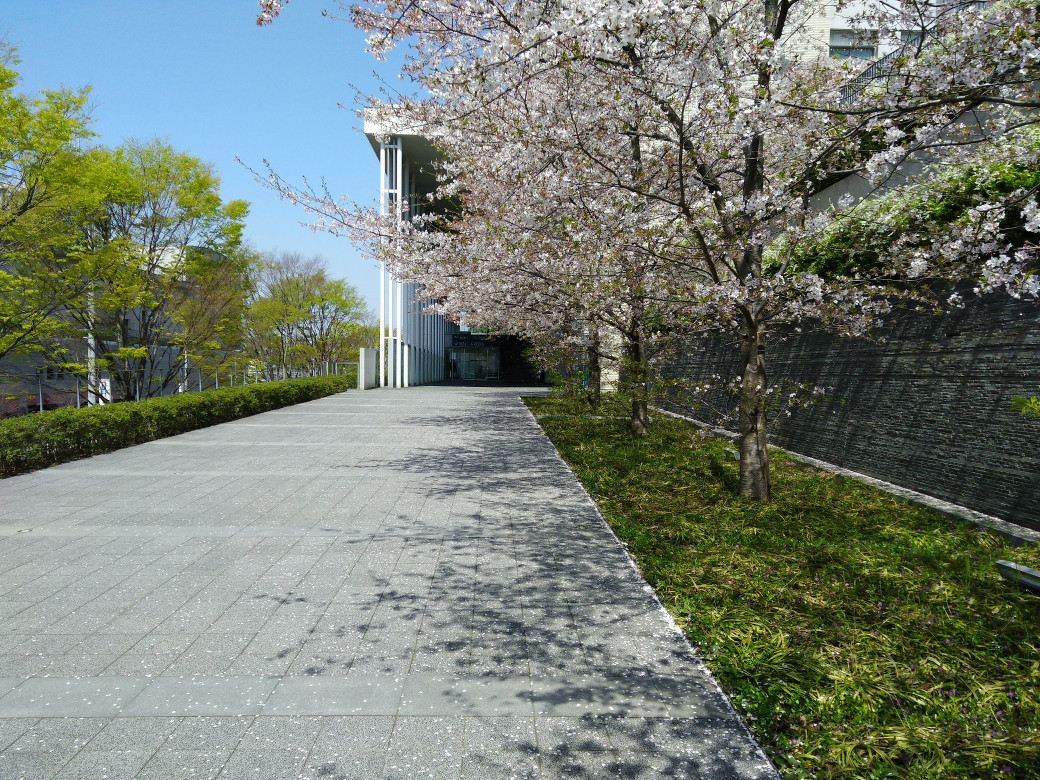
\includegraphics[clip,width=80mm]{img/sakura.jpg}
        \caption{卒業式の日吉キャンパスのオリジナル画像\label{fig:sakura}}
    \end{figure} 

    \begin{figure}[htbp]
        \begin{minipage}{0.5\hsize}
         \begin{center}
          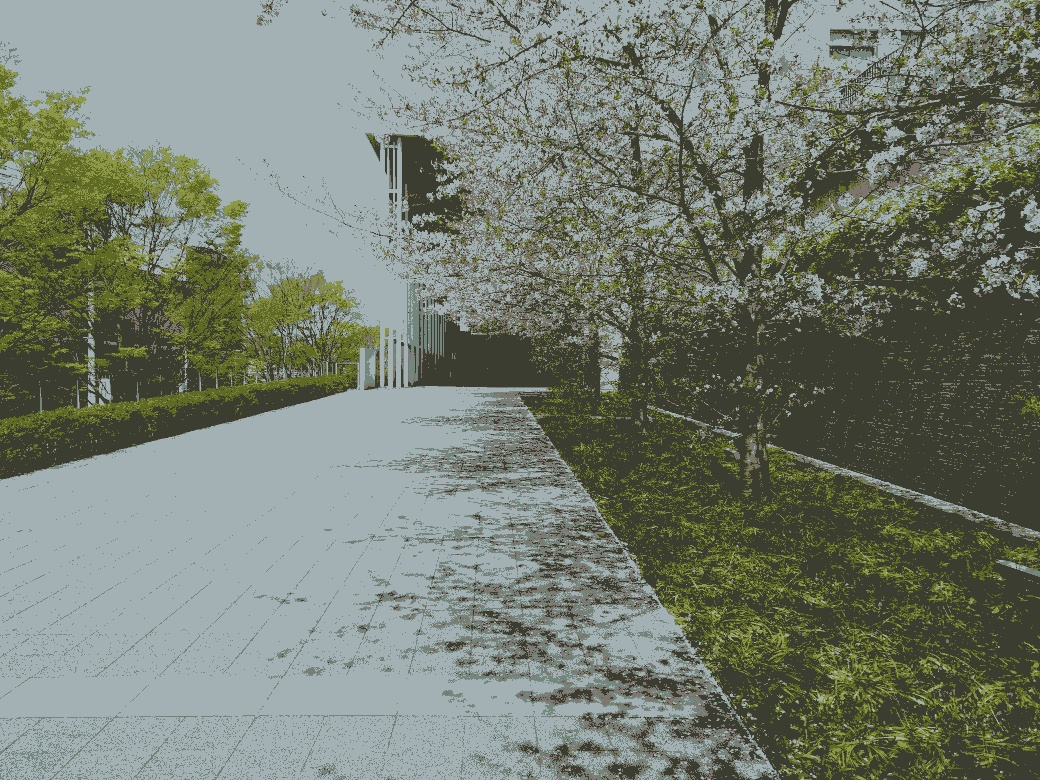
\includegraphics[width=80mm]{img/sakura_result.jpg}
         \end{center}
         \caption{卒業式の日吉キャンパス(自作k-means)}
        \end{minipage}
        \begin{minipage}{0.5\hsize}
         \begin{center}
          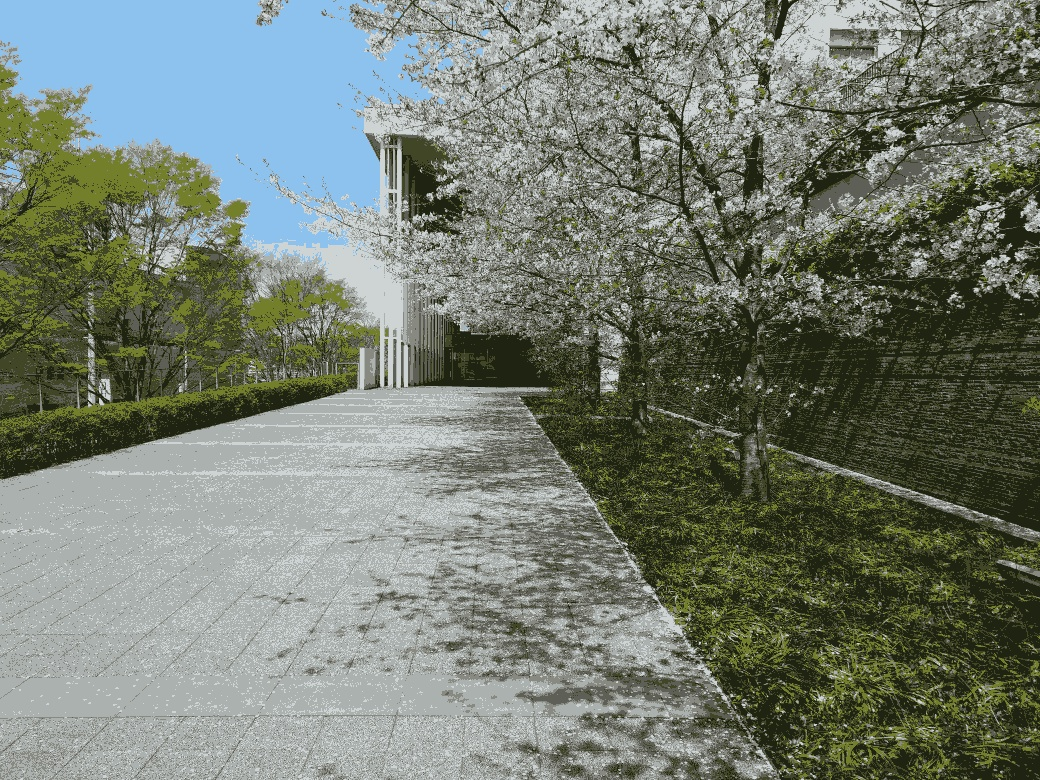
\includegraphics[width=80mm]{img/sakura_opencv.jpg}
         \end{center}
         \caption{卒業式の日吉キャンパス(cv2.kmeans)}
        \end{minipage}
    \end{figure} 
    次に今年の卒業式で撮影した桜の木の写真について見ていく。この場合はライブラリのもののほうがより明るい色となっている。
    自作のものについては空の青も保存されていない。

    \begin{figure}[H]
        \centering
        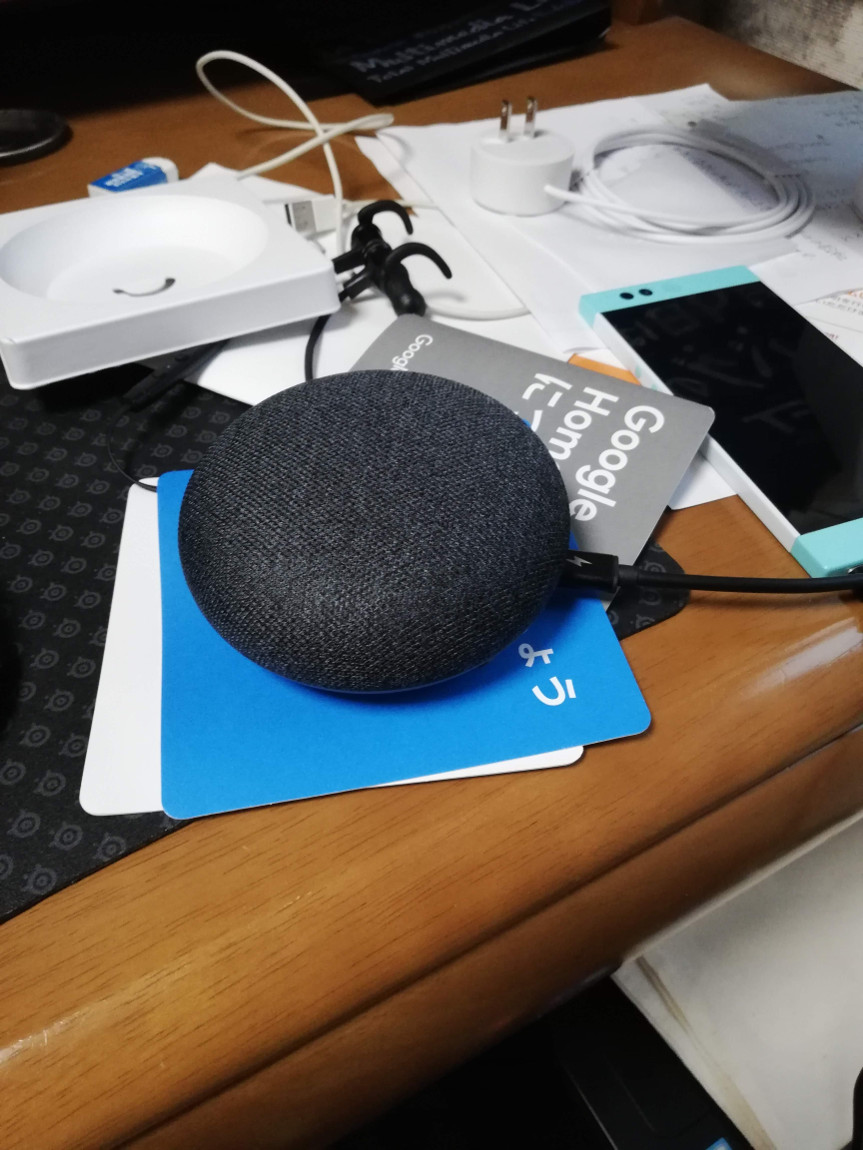
\includegraphics[clip,width=80mm]{img/mydesk.jpg}
        \caption{自宅の作業机のオリジナル画像\label{fig:mydesk}}
    \end{figure} 

    \begin{figure}[htbp]
        \begin{minipage}{0.5\hsize}
         \begin{center}
          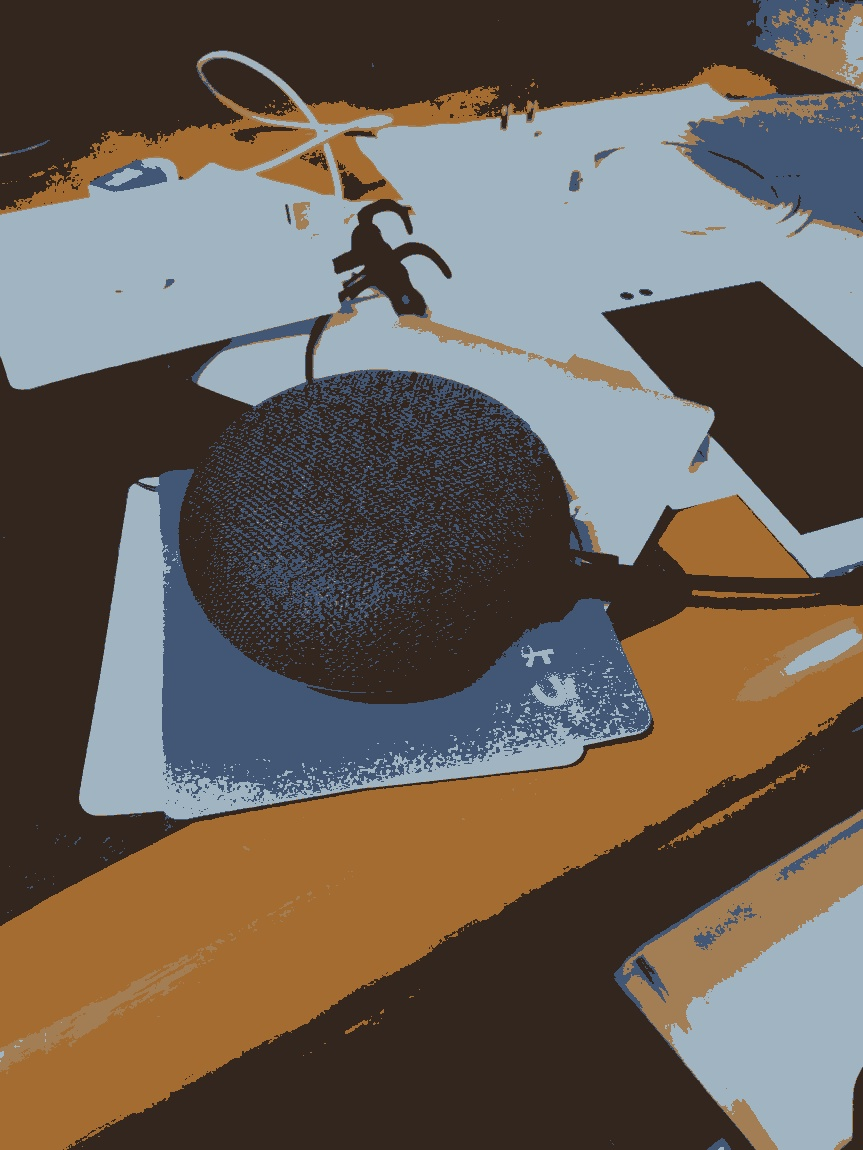
\includegraphics[width=80mm]{img/mydesk_result.jpg}
         \end{center}
         \caption{自宅の作業机(自作k-means)}
        \end{minipage}
        \begin{minipage}{0.5\hsize}
         \begin{center}
          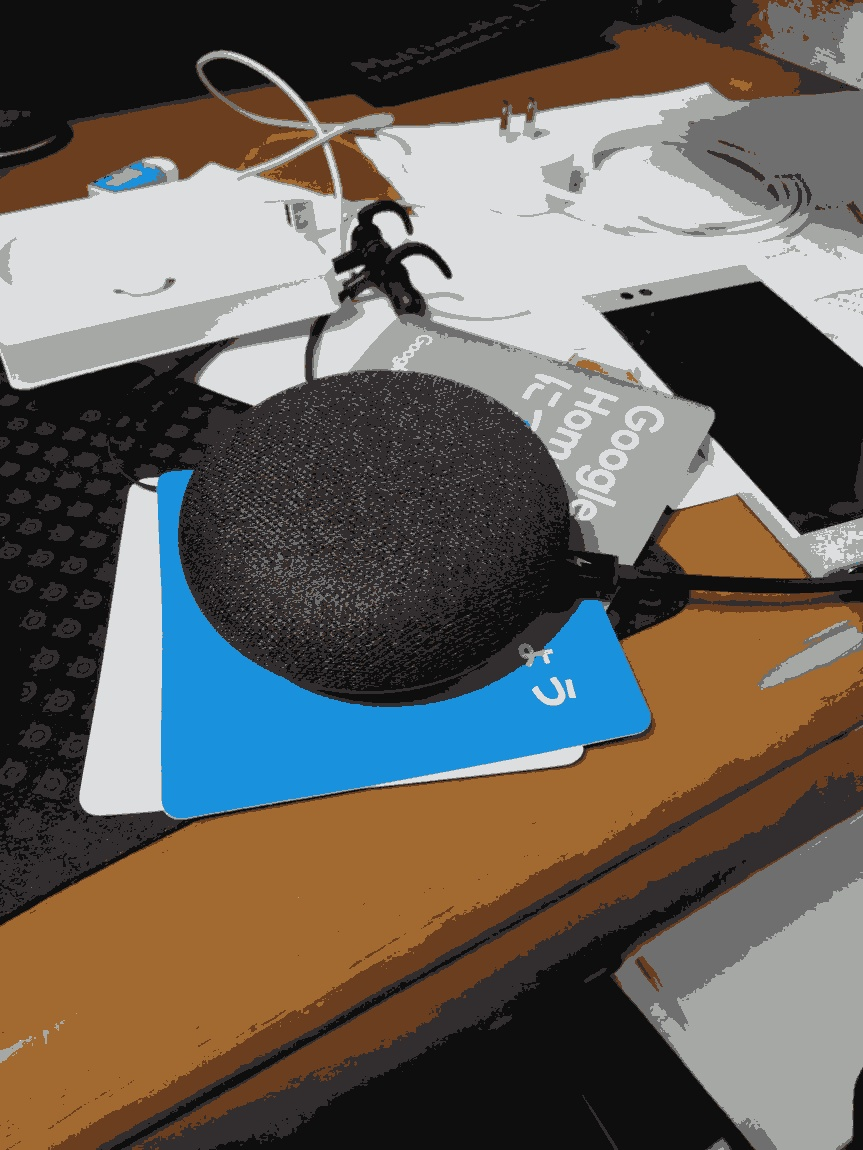
\includegraphics[width=80mm]{img/mydesk_opencv.jpg}
         \end{center}
         \caption{自宅の作業机(cv2.kmeans)}
        \end{minipage}
    \end{figure} 
    次に自宅の机の上を撮影した写真を見る。この画像がこのレポート中で一番ライブラリと自作のものについて大きな違いがある。
    スマートフォンの水色と紙の白が一体となってしまっている。画像の全体で比較的黒いものが多いので、そこにクラスタも引っ張られてしまっているように考える。
    マウスパッドの模様も自作のほうは消えてしまっている。
    
    \begin{figure}[H]
        \centering
        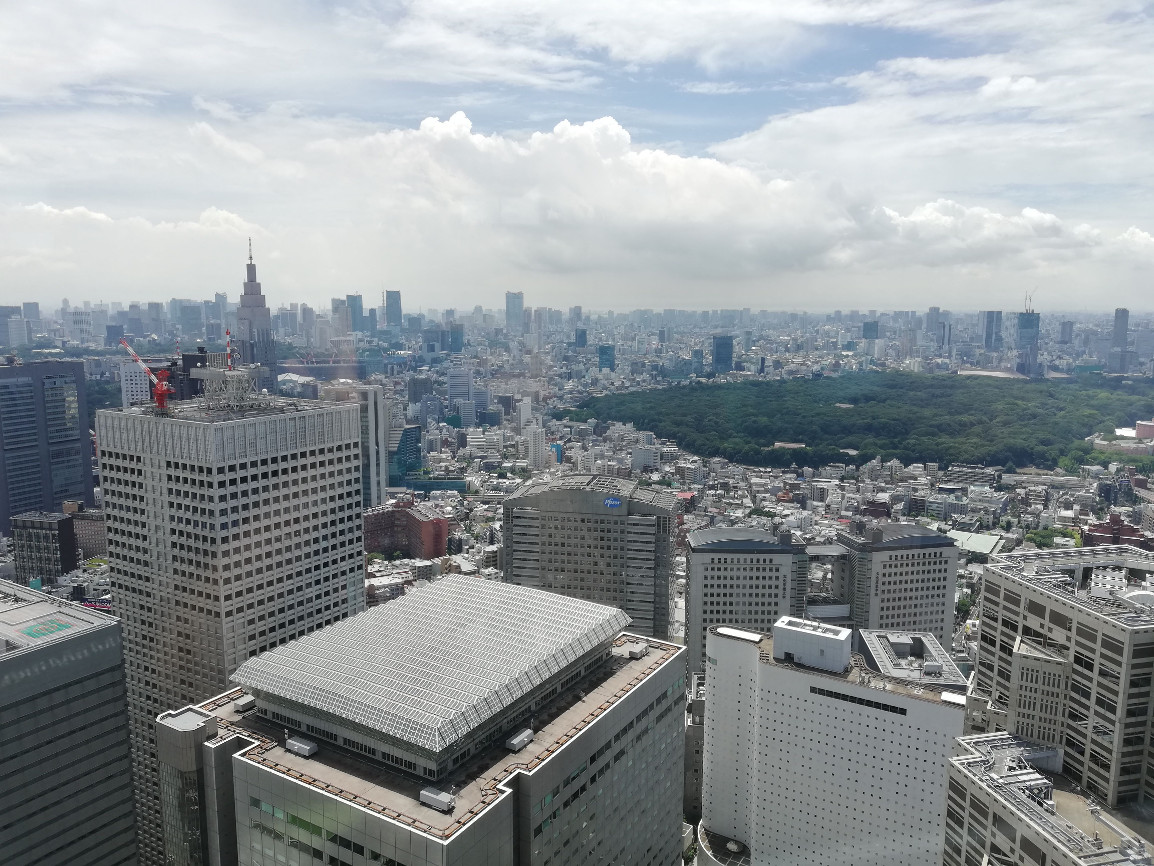
\includegraphics[clip,width=80mm]{img/metro.jpg}
        \caption{都庁展望台からの眺めのオリジナル画像\label{fig:metro}}
    \end{figure} 

    \begin{figure}[htbp]
        \begin{minipage}{0.5\hsize}
         \begin{center}
          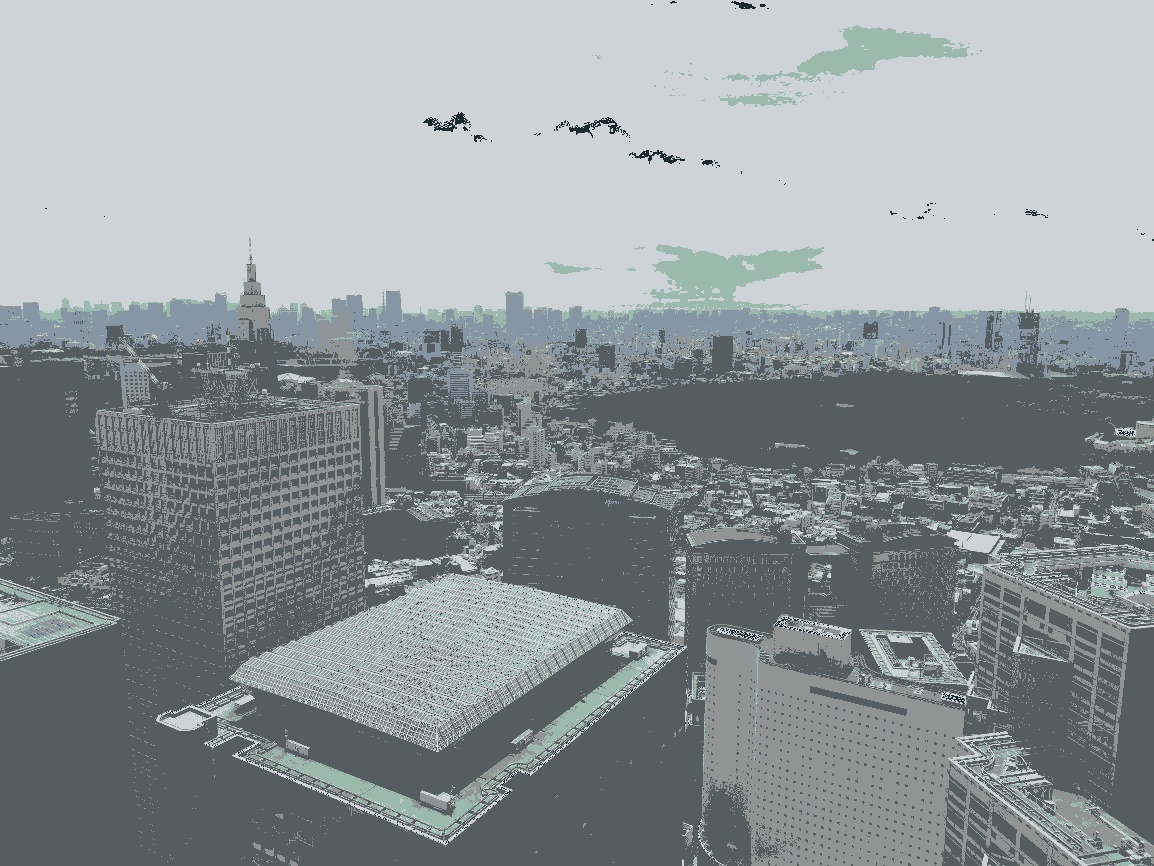
\includegraphics[width=80mm]{img/metro_result.jpg}
         \end{center}
         \caption{都庁展望台からの眺め(自作k-means)}
        \end{minipage}
        \begin{minipage}{0.5\hsize}
         \begin{center}
          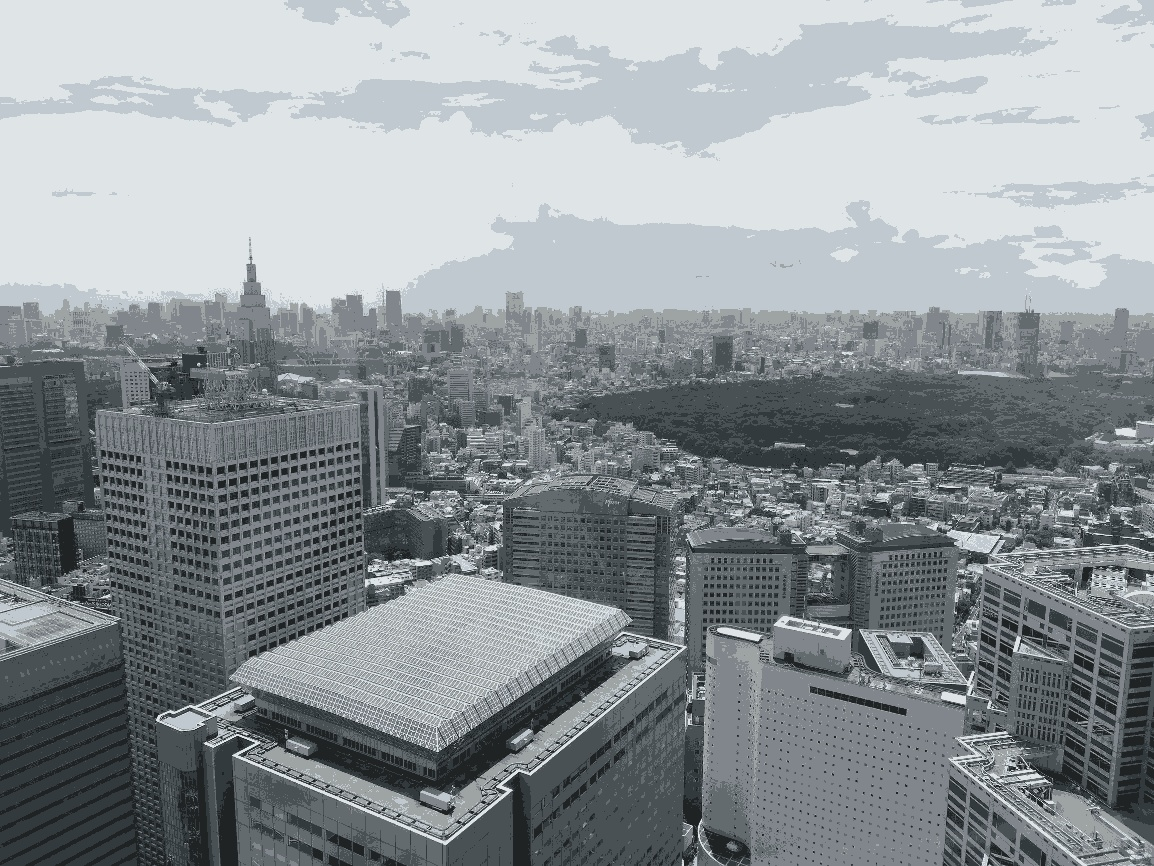
\includegraphics[width=80mm]{img/metro_opencv.jpg}
         \end{center}
         \caption{都庁展望台からの眺め(cv2.kmeans)}
        \end{minipage}
    \end{figure} 
    都庁の画像は比較的白っぽいビルの面積が多いので、そこまで差が出ないと予想していたがやはり自作のもののほうが色味が暗くなってしまい、
    ライブラリのほうが鮮明である。
    \section{混合ガウシアンモデルを用いたセグメンテーション}
    \subsection{混合ガウシアンモデルについて}
    混合ガウシアンモデルとは確率分布としてよく用いられるガウス分布の確率分布関数を複数重ね合わせたものである。

    具体例として、k-means同様に、ランダムに生成した2次元ベクトルを基にしてクラスタの重心を求めて、
    入力データがどのクラスタに属しているかを図\ref{fig:ex-gauss}に示す。
    バツマークがランダムに生成したベクトル、丸マークで示しているのが入力データである。
    ユークリッド距離が一番近いクラスタに分類されているのがわかる。


    \begin{figure}[H]
        \centering
        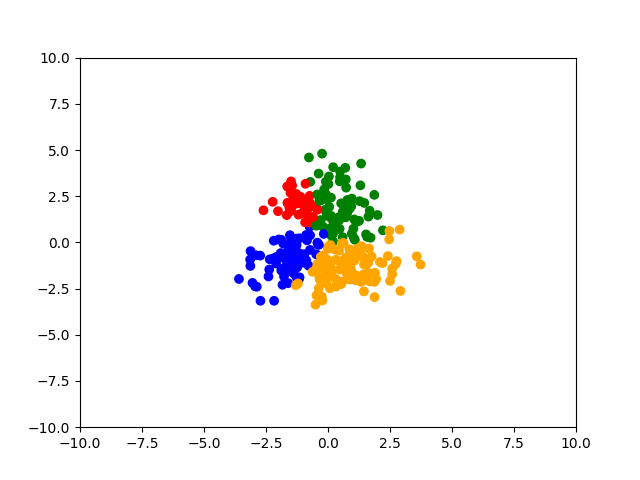
\includegraphics[clip,width=10.0cm]{img/gauss_5000.png}
        \caption{混合ガウシアンモデルによる2次元ベクトルのクラスタリングの様子\label{fig:ex-gauss}}
    \end{figure} 
    \subsection{実装方法}
    上図の2次元でのクラスタリングのためにNumpyで実装したコードのベクトルを3次元に拡張させて画像のセグメンテーションを行おうとしたが、
    上手く実装できなかった。

    \section{結論}
    セグメンテーションについてより詳しく知るためにk-means法を自分で実装してOpenCVライブラリの実装との比較を行った。
    力及ばず他のアルゴリズムについては検討できなかったが、実装が比較的単純なk-meansでもオリジナルの画像やライブラリの関数で処理したものと比べて上手くセグメンテーションができていない。
    原因として考えられるのは自分がプログラムを書く際にnumpyの挙動について、勉強不足で一部の途中の演算の処理でエラーが起きてしまったりしていることが要因と考えられる。
    
